% update_intense.tex — Полный текст секции 3.1 «Анализ индивидуальной селективности нейронов
% с помощью информационно-теоретических методов»
%
% ИНСТРУКЦИЯ: после ревью — заменить содержимое секции \ref{sec:intense} в part3.tex
% (строки 4–21) на содержимое этого файла.
%
% Описание эксперимента и данных вынесено в секцию 2.4.1 (update_nof.tex).
% Здесь только ссылка.
%
% Рисунки: images/intense/fig{1..4}_delegated.{pdf,png}

\section{Анализ индивидуальной селективности нейронов с помощью информационно-теоретических методов}\label{sec:intense}

\subsection{Постановка задачи выявления селективных нейронов}

Взаимосвязи между нейронной активностью и внешними переменными (поведение, окружающая среда) могут быть сложными и нелинейными. Помимо этого, внешние переменные гетерогенны (непрерывные и дискретные), а нейронная активность представлена сигналами различных типов (например, кальциевая флуоресценция и выделенные события). В связи с этим необходимы методы, не делающие дополнительных предположений о структуре взаимосвязи.

Большинство аналитических подходов исходит из заранее заданных категорий нейронной селективности~--- клетки места, клетки скорости, нейроны, селективные к задаче,~--- неявно предполагая, что перечень значимых типов селективности уже известен. Однако при естественном поведении активность нейрона может быть связана с переменными, не являющимися каноническими и не очевидными заранее. Поэтому анализ селективности продуктивно ставить как задачу систематического \textit{поиска} статистически обоснованных связей <<нейрон--переменная>>, а не подтверждения принадлежности нейронов к предопределённым типам.

\subsection{Общая схема метода}

Для количественной оценки индивидуальной нейронной селективности в данной работе был разработан фреймворк INTENSE (INformation-Theoretic Evaluation of Neuronal SElectivity)~--- инструмент с открытым исходным кодом, переосмысляющий анализ селективности в непрерывных данных кальциевого имиджинга как задачу поиска: вместо проверки соответствия нейронов заранее выбранным категориям INTENSE систематически выявляет разнообразные связи <<нейрон--переменная>> на основе эффективной оценки взаимной информации (ВИ). INTENSE обеспечивает информационно-теоретическую оценку селективности отдельных нейронов в масштабе сотен и тысяч нейронов с учётом временных задержек, гетерогенных поведенческих переменных и коррелированного пространства поведенческих признаков.

INTENSE работает непосредственно с сырыми сигналами кальциевой флуоресценции, устраняя необходимость деконволюции спайков (рис.~\ref{fig:intense_method}). В качестве основной меры используется взаимная информация~--- величина, которая улавливает любую статистическую зависимость, линейную или нелинейную, и обращается в нуль тогда и только тогда, когда переменные независимы~\cite{Shannon1948, Borst1999, Strong1998}. Статистическая значимость оценивается с помощью пермутационного тестирования на основе циклического сдвига с параметрическим моделированием $p$-значений. Систематическая оптимизация задержки позволяет учесть кинетику кальциевого индикатора, а также проспективное или ретроспективное кодирование.

\begin{figure}[!htbp]
  \centering
  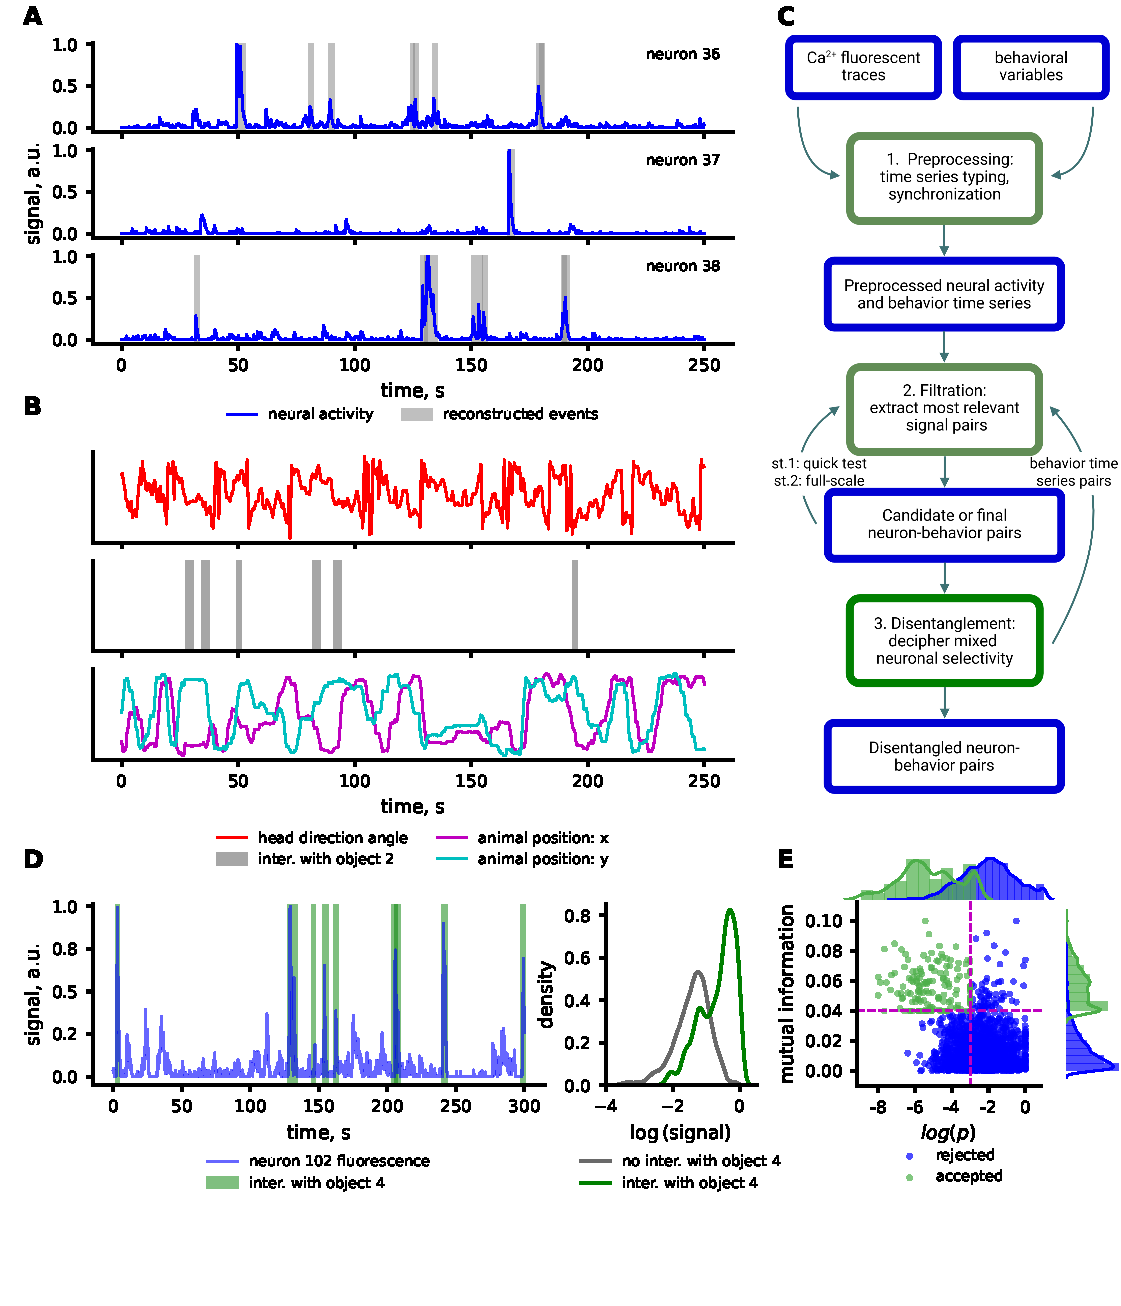
\includegraphics[width=0.85\linewidth]{images/intense/fig1_delegated.pdf}
  \caption{\textbf{A}: Примеры нормированных следов кальциевой флуоресценции $dF/F$ (синий) с детектированными событиями (серый).
\textbf{B}: Примеры поведенческих и средовых переменных: непрерывная (направление головы, вверху), дискретная (взаимодействие с объектом, середина), многомерная (координаты животного, внизу).
\textbf{C}: Схема конвейера INTENSE для количественной оценки нейронной селективности.
\textbf{D}: Слева: пример клетки, селективной к взаимодействию с объектом: след флуоресценции (синий) и периоды взаимодействия (зелёный). Справа: распределения нормированных значений $dF/F$ во время (зелёный) и вне (серый) периодов взаимодействия.
\textbf{E}: Распределение пар <<нейрон--поведение>> в пространстве <<значимость--сила эффекта>> с маргинальными распределениями. Пары, признанные значимыми, показаны зелёным}
  \label{fig:intense_method}
\end{figure}
\FloatBarrier

Помимо детекции, INTENSE предоставляет инструменты для анализа смешанной селективности. Многие нейроны гиппокампа и коры демонстрируют видимую селективность к нескольким поведенческим переменным одновременно~\cite{mix2,mix3}, однако отделение истинной смешанной селективности от корреляций, индуцированных ковариирующими поведенческими переменными, имеет принципиальное значение для понимания принципов нейронного кодирования и истинной размерности представлений. Процедура разделения запутанных селективностей, реализованная во фреймворке, использует условную ВИ и информацию взаимодействия~\cite{ghassami2017} для отделения подлинного многопеременного кодирования от ложных ассоциаций.

Описание экспериментальных данных приведено в секции~\ref{sec:nof_data}. Ниже последовательно описаны методы расчёта ВИ, статистического тестирования, разделения селективностей, а затем представлены результаты применения INTENSE к экспериментальным и синтетическим данным.


\subsection{Расчёт взаимной информации с помощью энтропии копулы}\label{sec:intense_gcmi}

Для оценки ВИ использовался метод взаимной информации на основе гауссовой копулы (Gaussian Copula Mutual Information, GCMI)~\cite{Ince2017, ma2011mutual}. Данный метод использует свойство, согласно которому взаимная информация зависит только от структуры зависимости (копулы) переменных, а не от их индивидуальных маргинальных распределений, что обеспечивает эффективное вычисление в замкнутой форме через ранговое преобразование. В отличие от гистограммных оценщиков, GCMI позволяет избежать проблемы выбора числа интервалов~\cite{Ross2014}; в отличие от оценщиков на основе $k$ ближайших соседей~\cite{Kraskov2004}, метод не требует большого объёма выборки. Он обеспечивает надёжную оценку ВИ как для пар непрерывных переменных, так и для пар <<дискретная--непрерывная>>.

Для двух случайных величин $X$ и $Y$ взаимная информация определяется как:
\begin{equation*}
I(X;Y) = H(X) + H(Y) - H(X,Y)
\end{equation*}

GCMI сначала преобразует переменные в пространство гауссовой копулы:
\begin{equation*}
\tilde{X} = \Phi^{-1}(F_X(X)), \quad \tilde{Y} = \Phi^{-1}(F_Y(Y))
\end{equation*}
где $F_X$ и $F_Y$~--- эмпирические функции распределения, а $\Phi^{-1}$~--- обратная функция стандартного нормального распределения.

\textbf{Случай <<непрерывная--непрерывная>>.} Для двух непрерывных переменных ВИ оценивается через корреляционную матрицу $\mathbf{R}$ преобразованных переменных:
\begin{equation*}
I_{GCMI}(X;Y) = -\frac{1}{2}\log_2|\mathbf{R}|
\end{equation*}

\textbf{Случай <<дискретная--непрерывная>>.} Для дискретной переменной $X$ с $K$ различными значениями и непрерывной переменной $Y$ ВИ вычисляется через разложение энтропии:
\begin{equation*}
I_{GCMI}(X;Y) = H(Y) - \sum_{k=1}^{K} p(X=k) \, H(Y | X=k)
\end{equation*}
где $H(Y)$~--- дифференциальная энтропия $Y$, оценённая методом GCMI, а каждая условная энтропия по классам $H(Y|X=k)$ оценивается по подмножеству данных, где $X = k$, с использованием предположения о гауссовой копуле.

Для каждой пары <<нейрон--поведенческая переменная>> сила селективности количественно оценивалась как:
\begin{equation*}
S = I(X_{\text{neural}}; Y_{\text{behavior}})
\end{equation*}


\subsection{Расчёт статистической значимости через генерацию синтетического распределения взаимной информации}\label{sec:intense_stat}

Для оценки значимости ВИ между кальциевой активностью и поведением наблюдаемое значение сравнивалось с нулевым распределением, построенным на основе данных со случайным временным сдвигом~\cite{skaggs1993information}. Нейронный сигнал $X(t)$ подвергался циклическому сдвигу на случайную величину $\tau_i$, после чего ВИ пересчитывалась:
$$MI_{\text{shuffle}}^{(i)} = I(X(t + \tau_i); Y(t))$$

Данная процедура повторялась многократно для построения нулевого распределения значений ВИ, ожидаемых при отсутствии связи. Циклический временной сдвиг сохраняет структуру временной автокорреляции, присущую как нейронным кальциевым сигналам, так и поведенческим переменным, при этом разрушая их временнýю связь~\cite{Lancaster2018}. Это принципиально важно, поскольку кальциевые индикаторы порождают сигналы с медленной динамикой (постоянные времени затухания 1--2~с для GCaMP6s)~\cite{Chen2013}, а поведенческие переменные часто демонстрируют сильные автокорреляции. Независимое сравнение статистических процедур для автокоррелированных данных кальциевого имиджинга~\cite{NevjenDunn2024} подтверждает этот выбор: пермутации на основе циклического сдвига обеспечивают наибольшую статистическую мощность при корректном контроле ошибки первого рода.

Полученное нулевое распределение моделировалось гамма-распределением с дополнительной массой в нуле (\textit{zero-inflated gamma distribution}):
$$P(MI = 0) = \pi, \quad P(MI = x \mid x > 0) = (1 - \pi) \cdot f_\Gamma(x; \alpha, \beta)$$
где $\pi$~--- параметр дополнительной массы в нуле, оценённый как доля значений ВИ при перемешивании, не превышающих $10^{-10}$, а $\alpha$ (форма) и $\beta$ (масштаб) оценивались методом максимального правдоподобия по ненулевым значениям ВИ при перемешивании. Выбор гамма-распределения обоснован: при справедливости нулевой гипотезы о независимости выборочная взаимная информация асимптотически распределена по закону $\chi^2$~\cite{Cover2006}, а $\chi^2$-распределение является частным случаем гамма-семейства; гамма-распределение также применялось напрямую для моделирования нулевых распределений ВИ в конечных выборках~\cite{hutter2001distribution}. Дополнительная масса в нуле учитывает точечную вероятность в нуле, возникающую у ранговых оценщиков при независимых переменных.

Значимость наблюдаемой ВИ оценивалась с помощью функции выживания подобранной модели:
$$p\text{-value} = (1 - \pi) \cdot [1 - F_\Gamma(MI_{\text{observed}}; \hat{\alpha}, \hat{\beta})]$$

\paragraph{Двухэтапная процедура тестирования.}

Для идентификации значимых пар <<нейрон--поведенческая переменная>> применялась двухэтапная процедура, обеспечивающая баланс между вычислительной эффективностью и контролем ложноположительных результатов.

\textbf{Этап~1. Скрининг.} Для каждой пары генерировалось 100 случайных перемешиваний; сохранялись пары, для которых $MI_{\text{observed}} > \max_{i=1}^{100} MI_{\text{shuffle}}^{(i)}$.

\textbf{Этап~2. Валидация.} Для сохранённых пар выполнялось 10\,000 дополнительных перемешиваний с применением двух критериев:
\begin{enumerate}
    \item \textbf{Непараметрический критерий}: $MI_{\text{observed}} > Q_{0.9995}(MI_{\text{shuffle}})$.
    \item \textbf{Параметрический критерий}: $p$-значение из подобранного гамма-распределения должно быть ниже скорректированного порога значимости.
\end{enumerate}

\paragraph{Ускорение пермутационного тестирования методом БПФ.}

Описанная двухэтапная процедура требует вычисления ВИ при тысячах циклических сдвигов для каждой пары. Наивная реализация имеет стоимость $O(n_{\text{sh}} \cdot n)$ на пару. Используется тот факт, что циклические временные сдвиги соответствуют циклическим кросс-корреляциям, которые для всех $n$ возможных сдвигов могут быть вычислены одновременно через теорему о свёртке:
\begin{equation}
\label{eq:fft_xcorr}
C_{XY}[s] = \sum_{i=0}^{n-1} X[i] \, Y[(i+s) \bmod n]
           = \mathcal{F}^{-1}\!\bigl[\mathcal{F}[X] \cdot \mathcal{F}[Y]^{*}\bigr][s]
\end{equation}
где $\mathcal{F}$ обозначает дискретное преобразование Фурье, а $^{*}$~--- комплексное сопряжение. Это снижает стоимость до $O(n \log n)$ для вычисления ВИ при всех сдвигах. Конкретная форма ВИ при каждом сдвиге зависит от типов переменных:

\textit{Случай <<непрерывная--непрерывная>>.} Для копула-нормализованных гауссовых переменных ВИ сводится к $I(X; Y_s) = -\tfrac{1}{2}\log_2(1 - r(s)^2)$, где $r(s)$~--- коэффициент корреляции Пирсона при сдвиге $s$, вычисляемый из ур.~\eqref{eq:fft_xcorr}.

\textit{Случай <<непрерывная--дискретная>>.} Для непрерывной переменной $Z$ и дискретной переменной $X$ с $K$ классами условные суммы по классам при каждом сдвиге представляют собой циклические корреляции с индикаторными функциями. Это требует $2K+2$ БПФ вне зависимости от числа перемешиваний.

\textit{Многомерный случай.} Для $d$-мерных поведенческих признаков (например, 2D-координаты положения) ковариационная матрица разделяется на инвариантные к сдвигу внутрипеременные блоки и зависящие от сдвига блоки кросс-ковариаций, вычисляемые с помощью $d$ БПФ.

INTENSE предвычисляет ВИ для всех $n$ сдвигов один раз для каждой пары и сохраняет результат в кэше. Суммарная стоимость составляет $O(N \cdot M \cdot n \log n)$ для построения кэша плюс $O(N \cdot M \cdot n_{\text{sh}})$ для выборки сдвигов~--- ускорение в $100$--$2500$ раз, что делает валидацию с 10\,000 перемешиваниями вычислительно выполнимой. На практике полный двухэтапный конвейер для 500 нейронов и 20 признаков при 10-минутной записи с частотой 20~кадров/с завершается приблизительно за 15~секунд.


\subsection{Применение поправок на множественные сравнения}\label{sec:intense_mc}

Порог $p$-значения определялся методом Холма--Бонферрони~\cite{Holm1979} для контроля семейной ошибки первого рода (FWER) на уровне $\alpha = 0{,}01$:
$$p_{\text{threshold}}^{(k)} = \frac{\alpha}{m - k + 1}$$
где $m$~--- число гипотез (пар, прошедших этап~1), а $k$~--- ранг упорядоченных $p$-значений. Контроль FWER, а не частоты ложных открытий (FDR), выбран как более консервативный: при поисковом анализе каждая отдельная связь <<нейрон--признак>> интерпретируется как самостоятельный биологический результат.

Дополнительно, для исключения пар с формально значимой, но слишком слабой связью применялся фиксированный порог силы эффекта: $MI_{\text{observed}} > MI_{\text{threshold}}$, где для анализируемого набора гиппокампальных записей $MI_{\text{threshold}} = 0{,}04$~бита (что соответствует ранговой корреляции Спирмена $\approx 0{,}23$ для GCMI-оценщика); при значениях ниже этого порога настройка нейрона при ручном просмотре визуально не идентифицировалась.

Совместное использование непараметрического (рангового) и параметрического критериев обеспечивает робастность: ранговый критерий защищает от ошибок подгонки распределения, типичных при наличии выбросов в биологических записях, тогда как параметрическое $p$-значение обеспечивает бóльшую статистическую мощность для обнаружения слабых, но устойчивых ассоциаций.

\paragraph{Оптимизация временной задержки.}

Для вычисления оптимальных задержек между нейронной активностью и поведением тестировался диапазон задержек от $-2$ до $+2$~с с шагом 0{,}05~с; выбиралась задержка, максимизирующая ВИ. Окно поиска $\pm 2$~с обосновано: (1)~максимальным горизонтом предсказания в навигационных задачах ($\sim$2~с)~\cite{Lian2022}; (2)~полным затуханием кальциевых транзиентов GCaMP6s ($\sim$2~с)~\cite{Zhang2023}; (3)~характерными поведенческими временными масштабами при принятии решений грызунами.


\subsection{Применение условной взаимной информации для задачи разделения нейронной селективности}\label{sec:intense_disentangle}

Когда несколько поведенческих переменных коррелированы, видимая нейронная селективность к одной переменной может возникать из-за её связи с другой~\cite{mix,mix3}. Для определения того, отражает ли перекрытие селективностей истинное совместное кодирование или избыточность переменных, к парам поведенческих переменных применялась та же процедура оценки значимости на основе ВИ. Если значимая ВИ между двумя поведенческими переменными не обнаруживалась, нейроны, селективные к обеим, считались независимо информативными.

В случае значимой связи между поведенческими переменными селективность дополнительно анализировалась с помощью условной взаимной информации (УВИ). Пусть $A$ обозначает нейронную активность, а $X$ и $Y$~--- две поведенческие переменные. Условная взаимная информация $I(A,X|Y)$ вычислялась в зависимости от типов $X$ и $Y$ (непрерывные, дискретные и их комбинации) с использованием соответствующих форм GCMI-оценщика.

Затем вычислялась информация взаимодействия (\textit{interaction information}, II)~\cite{McGill1954,ghassami2017}, количественно характеризующая избыточность или синергию в тройке $A$, $X$ и $Y$:
$$II(A,X,Y) = I(A;X|Y) - I(A;X)$$

Данная величина симметрична относительно трёх переменных. Ненулевое значение $|II|$ указывает на то, что три попарные связи не являются независимыми: отрицательные значения возникают, когда кондиционирование снижает взаимную информацию (избыточность), положительные~--- когда повышает (синергия)~\cite{Bell2003}.

Следуя~\cite{ghassami2017}, $|II|$ использовался как порог для выявления слабых информационных путей в рамках направленного ациклического графа. Попарная связь считалась <<слабой>>, если её ВИ была меньше $|II|$, что ограничивает топологию взаимодействия двумя возможными конфигурациями. Процедура определяет, какую из двух коррелированных переменных нейрон преимущественно кодирует, либо маркирует пару как неоднозначную при данном наборе переменных.


\subsection{Результаты анализа нейронной селективности в задаче обследования новой обстановки}\label{sec:intense_results}

INTENSE был применён к данным кальциевого имиджинга гиппокампа 16 мышей при свободном исследовании новой обстановки. Анализ организован как систематический поиск: сначала метод валидируется на канонической задаче детекции клеток места, затем применяется для непредвзятого обнаружения разнообразных селективностей, и наконец проверяется на синтетических данных с известным истинным ответом.

\subsubsection{Валидация INTENSE сопоставлением с методами детекции клеток места}

Для проверки точности INTENSE фреймворк был применён к хорошо изученной задаче идентификации клеток места (КМ)~--- нейронов, проявляющих селективность к определённым местоположениям в окружающей среде~\cite{o1971hippocampus}. Детекция КМ представляет собой требовательный критерий валидации, поскольку перекрытие между различными методами может составлять всего 30--40\%~\cite{Grijseels2021}.

Было проведено сравнение INTENSE, применённого непосредственно к сигналам кальциевой флуоресценции и координатам животного, с классическим методом на основе событий, строящим бинаризованные карты активности по деконвольвированным кальциевым событиям~\cite{skaggs1993information}.

\begin{figure}[!htbp]
  \centering
  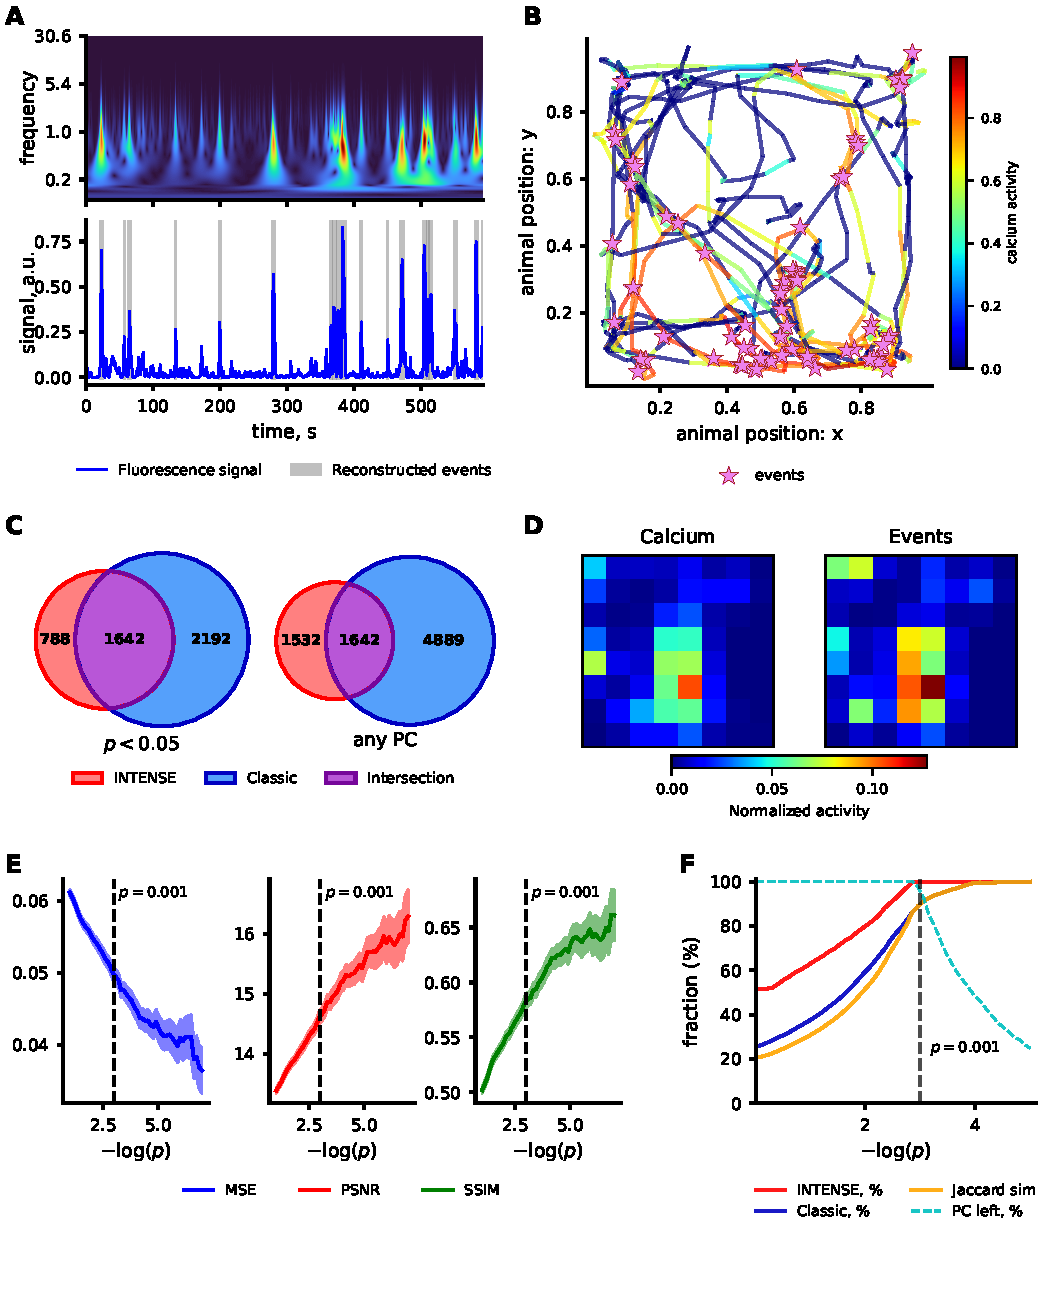
\includegraphics[width=0.85\linewidth]{images/intense/fig2_delegated.pdf}
  \caption{\textbf{A}: Вверху~--- карта непрерывного вейвлет-преобразования (CWT) сигнала флуоресценции. Внизу~--- след флуоресценции (синий) и детектированные события (серый).
\textbf{B}: Пример траектории животного, цветом показана нормированная кальциевая активность одной клетки места.
\textbf{C}: Пересечение популяций КМ, идентифицированных INTENSE и классическим методом.
\textbf{D}: Пример карт активности по сырым сигналам (слева) и по событиям (справа) с высоким показателем SSIM.
\textbf{E}: Метрики сходства между картами активности как функции уровня доверия ($p$-значение).
\textbf{F}: Относительное пересечение популяций КМ как функция уровня доверия}
  \label{fig:intense_pc}
\end{figure}
\FloatBarrier

Несмотря на умеренное перекрытие ($\sim$40\%) при учёте всех клеток, идентифицированных любым из методов, согласованность резко возрастала при применении порогов уверенности (рис.~\ref{fig:intense_pc}C). Перекрытие монотонно увеличивалось с ужесточением порога, достигая 90\% при $p < 0{,}001$~--- пороге, при котором сохранялось 95\% общей популяции КМ. Все метрики пространственного соответствия между картами активности улучшались с повышением порогов уверенности (рис.~\ref{fig:intense_pc}E), подтверждая, что КМ, идентифицированные с высокой уверенностью обоими методами, демонстрируют весьма сходные паттерны пространственной активности.

\subsubsection{Разнообразная нейронная селективность в гиппокампе}

После валидации INTENSE был применён для обнаружения ассоциаций между нейронной активностью и широким набором поведенческих признаков, включающим пространственное положение, направление головы, параметры движения и дискретные поведенческие состояния.

\begin{figure}[!htbp]
  \centering
  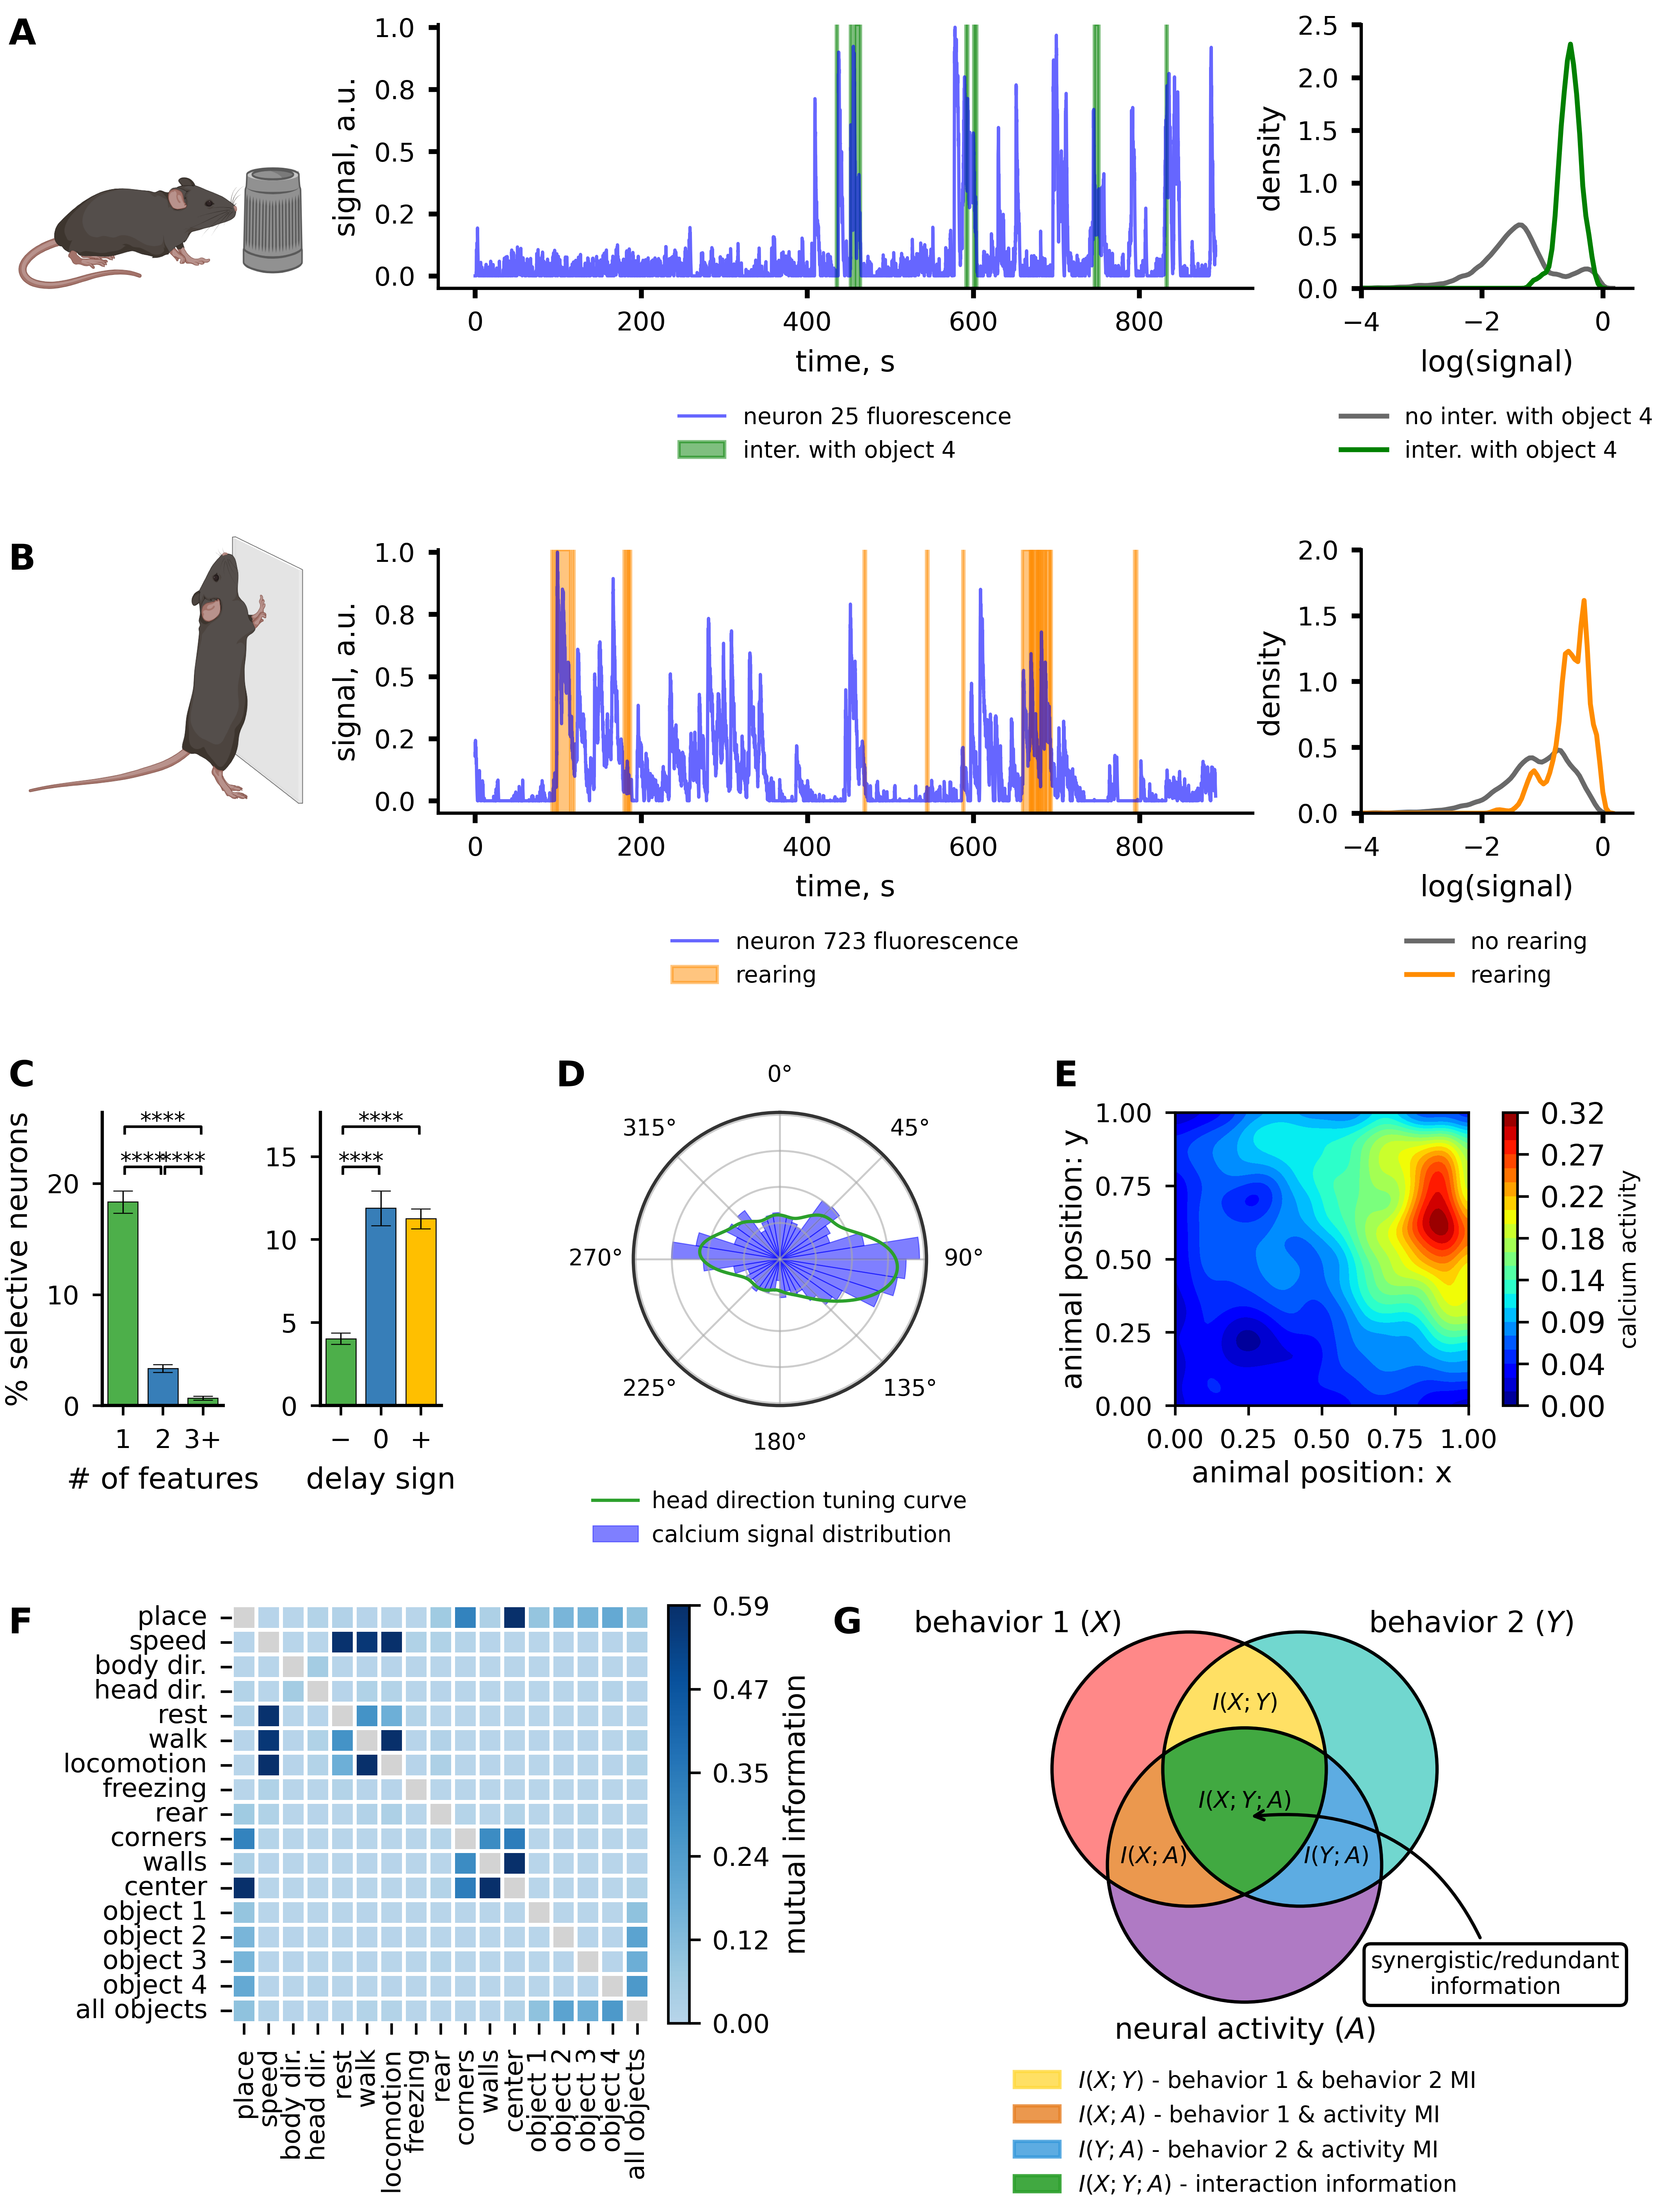
\includegraphics[width=0.85\linewidth]{images/intense/fig3_delegated.png}
  \caption{\textbf{A}: Пример <<нейрона взаимодействия с объектом>> и распределения $dF/F$.
\textbf{B}: Пример <<нейрона вставания на задние лапы>> и распределения $dF/F$.
\textbf{C}: Слева~--- распределение нейронов, селективных к 1--3 переменным. Справа~--- распределение оптимальных задержек.
\textbf{D}: Карта настройки на направление головы мультиселективного нейрона.
\textbf{E}: Двумерная карта пространственной активности того же нейрона.
\textbf{F}: Тепловая карта ВИ между статистически значимо коррелирующими поведенческими признаками.
\textbf{G}: Схема взаимозависимостей между информационными мерами для нейронов с запутанной селективностью}
  \label{fig:intense_results}
\end{figure}
\FloatBarrier

Результаты показали наличие множества нейронов, селективных к различным конкретным поведенческим признакам (рис.~\ref{fig:intense_results}A,B). Наряду с кодированием дискретных поведенческих актов были обнаружены многочисленные клетки, селективные к непрерывным переменным: скорости движения, направлению головы и пространственному положению (рис.~\ref{fig:intense_results}D,E).

\paragraph{Временное согласование нейронной активности и поведения.} Большинство значимых ассоциаций наблюдалось при положительных задержках (44{,}5\%), что согласуется с ожидаемым временным запаздыванием кальциевых индикаторов; 41{,}0\%~--- при околонулевых задержках и лишь 14{,}5\%~--- при отрицательных (рис.~\ref{fig:intense_results}C). Часть последних может отражать не артефакт, а подлинное проспективное кодирование. В дальнейшем анализе селективности, если не оговорено иное, рассматривались пары с неотрицательной оптимальной задержкой.

\paragraph{Количественная оценка и разделение смешанной селективности.} Из 30\,105 пар <<нейрон--сессия>>, проанализированных по 16 мышам и 4 сессиям, 6\,217 (20{,}7\%) показали значимую селективность хотя бы к одной поведенческой переменной. Среди них 1\,377 (22{,}1\% селективных нейронов) отвечали на две и более переменные до проведения процедуры разделения.

Процедура разделения на основе УВИ позволила разрешить существенную долю этих многопеременных ассоциаций. После контроля поведенческих корреляций число мультиселективных нейронов уменьшилось с 1\,377 до 949 (15{,}3\% от селективных); примерно треть многопеременных ассоциаций была объяснена поведенческой избыточностью. Наиболее выраженный эффект наблюдался для селективности к скорости: из 201 нейрона, первоначально классифицированного как селективный к скорости, лишь 7 сохранили значимость после кондиционирования на состояние локомоции. Этот результат воспроизводит давно отмеченную в гиппокампе тесную взаимосвязь скорости и локомоторного состояния, затрудняющую разделение их вкладов~\cite{Vanderwolf1969, McNaughton1983}, и служит положительным контролем корректности процедуры разделения. Вместе с тем этот пример очерчивает и границу применимости информационного скрининга: для столь тесно коррелированных переменных он практически не разделяет их вклады, и значимость к одной из них (скорости) почти полностью поглощается другой (локомоцией).

\paragraph{Взаимная информация выявляет ассоциации, невидимые для линейной корреляции.} При замене ВИ на корреляцию Пирсона в идентичном конвейере было выявлено в 2{,}2 раза меньше селективных нейронов и в 2{,}9 раза меньше значимых пар <<нейрон--признак>>. Наибольшее расхождение наблюдалось для дискретных поведенческих переменных (5--11$\times$).

\subsubsection{Валидация на синтетических данных}

Для строгой оценки детекционных возможностей INTENSE были проведены систематические испытания на синтетических наборах данных с известным истинным ответом. Генерировались эксперименты, содержащие 20 поведенческих временных рядов и 500 псевдокальциевых сигналов, причём каждый кальциевый сигнал был связан ровно с одной поведенческой переменной (распространённость истинных ассоциаций~--- 5\%). Варьировались отношение сигнал/шум (SNR $\in \{2, 4, 8, 16, 32, 64\}$) и надёжность ответа ($p_{\text{skip}} \in [0{,}0;\; 0{,}8]$).

\begin{figure}[!htbp]
  \centering
  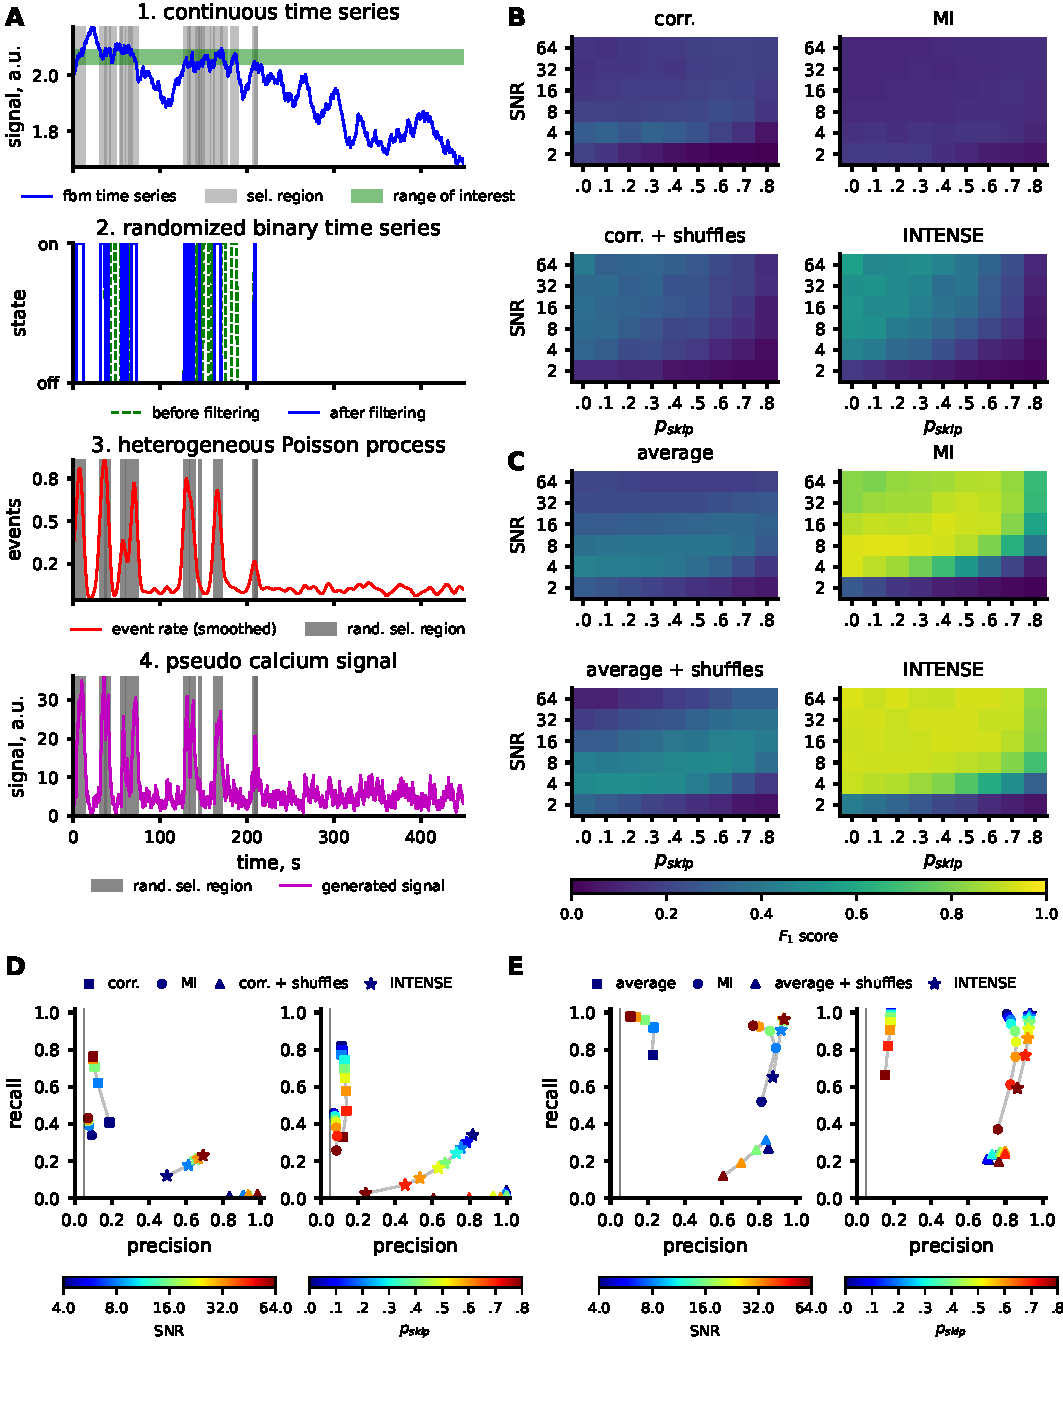
\includegraphics[width=0.85\linewidth]{images/intense/fig4_delegated.pdf}
  \caption{\textbf{A}: Этапы генерации псевдокальциевого сигнала, связанного с непрерывной переменной.
\textbf{B}: Тепловые карты F1-меры для непрерывных переменных: методы на основе корреляции, ВИ, корреляции с перемешиванием и INTENSE.
\textbf{C}: То же для дискретных переменных.
\textbf{D}: Карты <<точность--полнота>> для непрерывных переменных.
\textbf{E}: Карты <<точность--полнота>> для дискретных переменных}
  \label{fig:intense_synthetics}
\end{figure}
\FloatBarrier

Сравнение методов выявило фундаментальную проблему: без контроля временной автокорреляции методы на основе корреляции или ВИ достигали точности лишь 8{,}7\% и 6{,}4\% соответственно, что едва превышает 5\%-ный уровень случайного угадывания (рис.~\ref{fig:intense_synthetics}B--E).

Среди методов с контролем перемешиванием INTENSE продемонстрировал явные преимущества. При идеальной надёжности ответа точность возрастала с 44{,}2\% при SNR~=~2 до 85{,}5\% при SNR~=~64 для непрерывных переменных. Дискретные переменные дали существенно лучшие результаты: точность от 73{,}5\% до 94{,}6\%, полнота от 24{,}3\% до 100{,}0\%.

INTENSE также продемонстрировал робастность к эффектам насыщения кальциевого индикатора при высоких SNR, тогда как методы на основе сырой ВИ и средних значений показали деградацию характеристик. F1-мера INTENSE монотонно возрастала с 95{,}2\% до 97{,}2\%.

\subsection{Обсуждение}\label{sec:intense_discussion}

Фреймворк INTENSE объединяет оценку взаимной информации на основе гауссовой копулы с пермутационным тестированием на циклических сдвигах, что позволяет анализировать селективность непосредственно по сырой кальциевой флуоресценции, без деконволюции спайков. Принципиальная особенность подхода~--- постановка анализа как задачи поиска: его результатом является не перечень нейронов заранее известных типов, а структурированная карта статистически обоснованных связей <<нейрон--переменная>>, пригодная для последующей содержательной интерпретации.

Применение INTENSE к данным гиппокампа выявило две закономерности. Во-первых, лишь меньшинство нейронов оказалось селективно к каждой отдельной переменной, что согласуется с представлениями о разреженности нейронного кодирования. Во-вторых, около трети видимой мультиселективности объясняется не истинным совместным кодированием, а ковариацией поведенческих переменных; следовательно, оценки смешанной селективности, полученные без явного контроля поведенческих корреляций, систематически её завышают. Замена взаимной информации на линейную корреляцию в том же конвейере приводит к потере около двух третей значимых связей: существенная доля зависимостей <<нейрон--поведение>> нелинейна и невидима для линейных мер~--- это согласуется с искривлённостью многообразий нейронной активности, обсуждаемой в секции~\ref{sec:dim}.

Метод имеет ряд ограничений. Процедура разделения селективности контролирует только измеренные поведенческие переменные, поэтому неучтённые факторы могут порождать остаточные ложные ассоциации; кроме того, при фиксированном расположении объектов в арене селективность к месту и к объекту принципиально неразделима. Оценщик GCMI улавливает преимущественно монотонные зависимости, и немонотонная настройка нейронов может недооцениваться; непараметрические оценщики (метод $k$ ближайших соседей) свободны от этого ограничения, но требуют существенно больших объёмов выборки. Наконец, информационно-теоретический анализ остаётся вычислительно затратным при росте числа нейронов и переменных, что лишь частично смягчается двухэтапной процедурой тестирования.

